\iffalse
\let\negmedspace\undefined
\let\negthickspace\undefined
\documentclass[journal,12pt,twocolumn]{IEEEtran}

\usepackage{cite}
\usepackage{amsmath,amssymb,amsfonts,amsthm}
\usepackage{algorithmic}
\usepackage{graphicx}
\usepackage{textcomp}
\usepackage{xcolor}
\usepackage{txfonts}
\usepackage{listings}
\usepackage{enumitem}
\usepackage{mathtools}
\usepackage{gensymb}
\usepackage[breaklinks=true]{hyperref}
\usepackage{tkz-euclide} % loads  TikZ and tkz-base
\usepackage{listings}
\usepackage{circuitikz}
\usepackage{graphicx}

%\newcounter{MYtempeqncnt}
\DeclareMathOperator*{\Res}{Res}
%\renewcommand{\baselinestretch}{2}
\renewcommand\thesection{\arabic{section}}
\renewcommand\thesubsection{\thesection.\arabic{subsection}}
\renewcommand\thesubsubsection{\thesubsection.\arabic{subsubsection}}

\renewcommand\thesectiondis{\arabic{section}}
\renewcommand\thesubsectiondis{\thesectiondis.\arabic{subsection}}
\renewcommand\thesubsubsectiondis{\thesubsectiondis.\arabic{subsubsection}}

% correct bad hyphenation here
\hyphenation{op-tical net-works semi-conduc-tor}
\def\inputGnumericTable{}                                 %%

\lstset{
	frame=single,
	breaklines=true,
	columns=fullflexible
}



\newtheorem{theorem}{Theorem}[section]
\newtheorem{problem}{Problem}
\newtheorem{proposition}{Proposition}[section]
\newtheorem{lemma}{Lemma}[section]
\newtheorem{corollary}[theorem]{Corollary}
\newtheorem{example}{Example}[section]
\newtheorem{definition}[problem]{Definition}
\newcommand{\BEQA}{\begin{eqnarray}}
	\newcommand{\EEQA}{\end{eqnarray}}
\newcommand{\define}{\stackrel{\triangle}{=}}
\newcommand\figref{Fig.~\ref}
\newcommand\tabref{Table~\ref}
\bibliographystyle{IEEEtran}
%\bibliographystyle{ieeetr}


\providecommand{\mbf}{\mathbf}
\providecommand{\pr}[1]{\ensuremath{\Pr\left(#1\right)}}
\providecommand{\qfunc}[1]{\ensuremath{Q\left(#1\right)}}
\providecommand{\sbrak}[1]{\ensuremath{{}\left[#1\right]}}
\providecommand{\lsbrak}[1]{\ensuremath{{}\left[#1\right.}}
\providecommand{\rsbrak}[1]{\ensuremath{{}\left.#1\right]}}
\providecommand{\brak}[1]{\ensuremath{\left(#1\right)}}
\providecommand{\lbrak}[1]{\ensuremath{\left(#1\right.}}
\providecommand{\rbrak}[1]{\ensuremath{\left.#1\right)}}
\providecommand{\cbrak}[1]{\ensuremath{\left\{#1\right\}}}
\providecommand{\lcbrak}[1]{\ensuremath{\left\{#1\right.}}
\providecommand{\rcbrak}[1]{\ensuremath{\left.#1\right\}}}
\theoremstyle{remark}
\newtheorem{rem}{Remark}
\newcommand{\sgn}{\mathop{\mathrm{sgn}}}
\providecommand{\abs}[1]{\left\vert#1\right\vert}
\providecommand{\res}[1]{\Res\displaylimits_{#1}}
\providecommand{\norm}[1]{\left\lVert#1\right\rVert}
%\providecommand{\norm}[1]{\lVert#1\rVert}
\providecommand{\mtx}[1]{\mathbf{#1}}
\providecommand{\mean}[1]{E\left[ #1 \right]}
\providecommand{\fourier}{\overset{\mathcal{F}}{ \rightleftharpoons}}
%\providecommand{\hilbert}{\overset{\mathcal{H}}{ \rightleftharpoons}}
\providecommand{\system}{\overset{\mathcal{H}}{ \longleftrightarrow}}
%\newcommand{\solution}[2]{\textbf{Solution:}{#1}}
\newcommand{\solution}{\noindent \textbf{Solution: }}
\newcommand{\cosec}{\,\text{cosec}\,}
\providecommand{\dec}[2]{\ensuremath{\overset{#1}{\underset{#2}{\gtrless}}}}
\newcommand{\myvec}[1]{\ensuremath{\begin{pmatrix}#1\end{pmatrix}}}
\newcommand{\mydet}[1]{\ensuremath{\begin{vmatrix}#1\end{vmatrix}}}
\renewcommand{\abstractname}{Question}

\let\vec\mathbf

	
	\vspace{3cm}
	
	


\newcommand{\permcomb}[4][0mu]{{{}^{#3}\mkern#1#2_{#4}}}
\newcommand{\comb}[1][-1mu]{\permcomb[#1]{C}}

%\IEEEpeerreviewmaketitle

\newcommand \tab [1][1cm]{\hspace*{#1}}
%\newcommand{\Var}{$\sigma ^2$}
\usepackage{amssymb}
\usepackage{amsmath}
\title{
	
\title{NCERT Physics 12.7 Q6}
\author{EE23BTECH11061 - SWATHI DEEPIKA$^{*}$% <-this % stops a space
}


}
\begin{document}

\maketitle

\textbf{Question:} 
Obtain the resonance frequency of a series LCR circuit with $L = 2.0\, H$, $C = 32\, \mu F$, and $R = 10\, \Omega$. What is the Q-value of the circuit.\\

\begin{figure}[!h]
	\centering
	
\begin{circuitikz}
    \draw(0, 0) -- (1, 0);
    \draw(1, 0) to [L, l = $2.0\text{H}$](2, 0);
    \draw(2, 0) -- (3, 0);
    \draw(3, 0) to [C, l = $32\, \mu\text{F}$](4, 0);
    \draw(4, 0) -- (5, 0);
    \draw(5, 0) to [R, l = $10\Omega$](6, 0);
    \draw(0, 0) -- (0, -2);
    \draw[->] (0, -1) node[left] {$I(t)$} -- (0, -1);
    \draw(6, 0) -- (7, 0);
    \draw(7, 0) -- (7, -2);
    \draw(0, -2) -- (3, -2);
    \draw(7, -2) -- (7, -2);
    \draw(3, -2) to [sV, l = $V(t)$](4, -2);
    \draw(4, -2) -- (7, -2);
\end{circuitikz}

	\caption{LCR Circuit}
\end{figure}
     
\textbf{Solution: }
\fi
 \begin{table}[h]
 	\centering
 	\resizebox{6 cm}{!}{
 		

\begin{tabular}{|c|c|c|}
    \hline
     \textbf{Symbol} & \textbf{Value} &
     \textbf{Description}\\
    \hline
     $L$ &  $2.0\ H$ & Inductance\\[6pt]
    \hline 
     $C$ &  $32\ \mu F$ & Capacitance \\[6pt]
    \hline
     $R$ &  $10\ \Omega$ & Resistance\\[6pt]
    \hline
     $Q$ & $\frac{V_L}{V_R}$ & Quality Factor\\[6pt]
    \hline
    $V_L$ & $sLI(j\omega)$ & Voltage across inductance\\[6pt]
    \hline
    $V_C$ & $RI(j\omega)$ & Voltage across capacitor\\[6pt]
    \hline
    $\omega_0$ & $\dfrac{1}{\sqrt{LC}}$ & Resonant frequency\\[6pt]
    \hline
\end{tabular}

 	}
 	\vspace{6 pt}
 	\caption{Parameters}
 \end{table}
 
\begin{figure}[!h]
 \centering
    \begin{circuitikz}
    \draw(0, 0) -- (1, 0);
    \draw(1, 0) to [L, l = $j\omega L$](2, 0);
    \draw(2, 0) -- (3, 0);
    \draw(3, 0) to [C, l = $\frac{1}{j\omega C}$](4, 0);
    \draw(4, 0) -- (5, 0);
    \draw(5, 0) to [R, l = $R$](6, 0);
    \draw(0, 0) -- (0, -2);
    \draw[->] (0, -1) node[left] {$I(j\omega)$} -- (0, -1);
    \draw(6, 0) -- (7, 0);
    \draw(7, 0) -- (7, -2);
    \draw(0, -2) -- (3, -2);
    \draw(7, -2) -- (7, -2);
    \draw(3, -2) to [sV, l = $V(j\omega)$](4, -2);
    \draw(4, -2) -- (7, -2);
\end{circuitikz}

    \caption{LCR Circuit}
\end{figure}

\begin{enumerate}
\item {Frequency Response of the Circuit}
\begin{align}
   V(j\omega) &= I(j\omega)\left(R + Lj\omega + \dfrac{1}{j\omega C}\right)\\
    \implies I(j\omega) &= \dfrac{V(s)}{\left(R + Lj\omega + \dfrac{1}{j\omega C}\right)}
\end{align}
At resonance,
\begin{align}
    Lj\omega + \dfrac{1}{j\omega C} &= 0
\end{align}
\begin{equation}
    \omega = \dfrac{1}{\sqrt{LC}}
\end{equation}

At resonance, Resonant frequency($\omega_0$) = $\dfrac{1}{\sqrt{LC}}$
\item{Quality Factor}

\begin{enumerate}
\item voltage across inductor,
\begin{align}
    Q &= \left(\dfrac{V_L}{V_R}\right)_{\omega_0} = \dfrac{\lvert{j\omega_0 LI(j\omega)}\rvert}{\lvert RI(j\omega) \rvert}\\
    &= \dfrac{1}{\sqrt{LC}}\dfrac{L}{R}\\
    &= \dfrac{1}{R}\sqrt{\dfrac{L}{C}}
\end{align}
\item Using voltage across capacitor,
\begin{align}
	Q &= \left(\dfrac{V_C}{V_R}\right)_{\omega_0} = \dfrac{\abs{\frac{I(j\omega)}{j\omega_0 C}}}{\lvert RI(j\omega) \rvert}\\
    &= \dfrac{\sqrt{LC}}{RC}\\
    &= \dfrac{1}{R}\sqrt{\dfrac{L}{C}}
\end{align}
\end{enumerate}
\item{Plot of Impedance vs Angular Frequency}
\begin{equation}
    H(j\omega) = \dfrac{V(j\omega)}{I(j\omega)}
\end{equation}

\begin{align}
      H(j\omega) &= R + j\omega L + \dfrac{1}{j\omega C}\\
     \implies \lvert H(j\omega) \rvert &= \sqrt{R^2 + \left(\omega L - \dfrac{1}{\omega C}\right)^2}
\end{align}
\begin{figure}[!h]
    \centering
    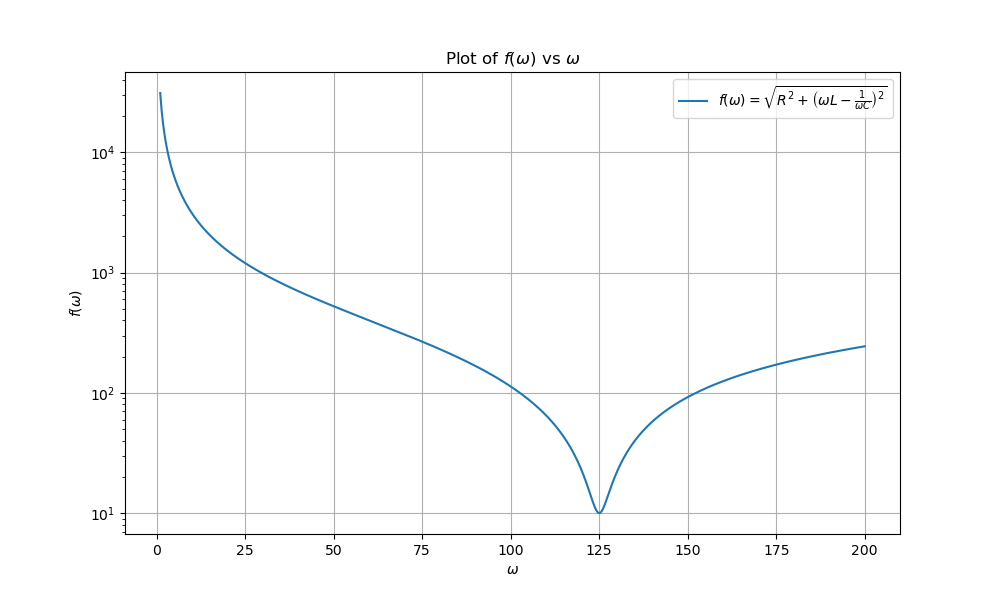
\includegraphics[width = \columnwidth]{ncert-physics/12/7/6/figs/q_plot.png}
    \caption{Impedance vs $\omega$ }
\end{figure}
\end{enumerate}

Substituting values,
\begin{align}
\omega_0 &= \dfrac{1}{\sqrt{(2.0)(32 \times 10^{-6})}}
\end{align}
\begin{align}
\omega_0 &= 125 \text{ Hz}
\end{align}


\begin{align}
Q &= \frac{1}{10}\sqrt{\frac{2}{32 \times 10^{-6}}}
\end{align}
\begin{align}
Q &= 25
\end{align}


%\end{document}



